\documentclass[paper=a4, fontsize=11pt]{scrartcl} % A4 paper and 11pt font size

%----------------------------------------------------------------------------------------
%	PACKAGES
%----------------------------------------------------------------------------------------
\usepackage[T1]{fontenc} % Use 8-bit encoding that has 256 glyphs
\usepackage{fourier} % Use the Adobe Utopia font for the document - comment this line to return to the LaTeX default
\usepackage[english]{babel} % English language/hyphenation
\usepackage{amsmath,amsfonts,amsthm} % Math packages
\usepackage{sectsty} % Allows customizing section commands
\usepackage{fancyhdr} % Custom headers and footers
\usepackage{xcolor} % Allows 0-255 RGB values
\usepackage{tabularx, outlines, framed, varwidth, enumitem, graphicx, listings, color, qtree, float, subcaption, newfloat, pdfpages}
\usepackage[left=0.5in, right=0.5in, top=3in, bottom=.25in]{geometry}
\geometry{}

%----------------------------------------------------------------------------------------
%	SET CUSTOMIZATIONS AND FUNCTIONS
%----------------------------------------------------------------------------------------
\sectionfont{\centering \normalfont\scshape} % Make all sections centered, the default font and small caps
\pagestyle{fancyplain} % Makes all pages in the document conform to the custom headers and footers
\fancyhead{} % No page header - if you want one, create it in the same way as the footers below
\fancyfoot[L]{} % Empty left footer
\fancyfoot[C]{} % Empty center footer
\fancyfoot[R]{\thepage} % Page numbering for right footer
\renewcommand{\headrulewidth}{0pt} % Remove header underlines
\renewcommand{\footrulewidth}{0pt} % Remove footer underlines
\setlength{\headheight}{0pt} % Customize the height of the header

\DeclareFloatingEnvironment[fileext=lod]{diagram}

\numberwithin{equation}{section} % Number equations within sections (i.e. 1.1, 1.2, 2.1, 2.2 instead of 1, 2, 3, 4)
\numberwithin{figure}{section} % Number figures within sections (i.e. 1.1, 1.2, 2.1, 2.2 instead of 1, 2, 3, 4)
\numberwithin{table}{section} % Number tables within sections (i.e. 1.1, 1.2, 2.1, 2.2 instead of 1, 2, 3, 4)

\graphicspath{{./figures/}}
%\setlength\parindent{0pt} % Removes all indentation from paragraphs - comment this line for an assignment with lots of text

\makeatletter
	\newcommand*\variableheghtrulefill[1][.4\p@]
	{%
		\leavevmode
		\leaders \hrule \@height #1\relax \hfill
		\null
	}
\makeatother

\definecolor{solBase03}{RGB}{000,043,054}
\definecolor{solBase02}{RGB}{007,054,066}
\definecolor{solBase01}{RGB}{088,110,117}
\definecolor{solBase00}{RGB}{101,123,131}
\definecolor{solBase0}{RGB}{131,148,150}
\definecolor{solBase1}{RGB}{147,161,161}
\definecolor{solBase2}{RGB}{238,232,213}
\definecolor{solBase3}{RGB}{253,246,227}
\definecolor{solYellow}{RGB}{181,137,000}
\definecolor{solOrange}{RGB}{203,075,022}
\definecolor{solRed}{RGB}{220,050,047}
\definecolor{solMagenta}{RGB}{211,054,130}
\definecolor{solViolet}{RGB}{108,113,196}
\definecolor{solBlue}{RGB}{038,139,210}
\definecolor{solCyan}{RGB}{042,161,152}
\definecolor{solGreen}{RGB}{133,153,000}

\lstdefinestyle{mystyle}{
	% To Match
	sensitive=true,	
	%
	% Add border
	frame=lines,
	%
	% Add Margin
	xleftmargin=\parindent,
	%
	% Put extra space under caption
 belowcaptionskip=1\baselineskip,
 %
 % Colors:
	backgroundcolor=\color{solBase3},
 basicstyle=\color{solBase00}\footnotesize,
 keywordstyle=\color{solCyan},
 commentstyle=\color{solBase1},
 stringstyle=\color{solBlue},
 numberstyle=\color{solViolet},
 identifierstyle=\color{solBase00},
 %
 % Formatting Options
 breakatwhitespace=false,
 breaklines=true, % break long lines
 captionpos=b,
 keepspaces=true,
 numbers=left,
 numbersep=5pt,
 showspaces=false,
 showstringspaces=false,
 showtabs=false,
 tabsize=4
}

\lstdefinestyle{smallstyle}{
	% To Match
	sensitive=true,	
	%
	% Add border
	frame=lines,
	%
	% Add Margin
	xleftmargin=\parindent,
	%
	% Put extra space under caption
 belowcaptionskip=1\baselineskip,
 %
 % Colors:
	backgroundcolor=\color{solBase3},
 basicstyle=\color{solBase00}\scriptsize,
 keywordstyle=\color{solCyan},
 commentstyle=\color{solBase1},
 stringstyle=\color{solBlue},
 numberstyle=\color{solViolet},
 identifierstyle=\color{solBase00},
 %
 % Formatting Options
 breakatwhitespace=false,
 breaklines=false, % break long lines
 captionpos=b,
 keepspaces=true,
 numbers=left,
 numbersep=5pt,
 showspaces=false,
 showstringspaces=false,
 showtabs=false,
 tabsize=2
}
 
\lstset{style=mystyle}

%----------------------------------------------------------------------------------------
%	USEFUL COMMANDS
%----------------------------------------------------------------------------------------
%	\makebox[\textwidth][c]{\includegraphics[width=.7\paperwidth]{p2-table}}

%	\newgeometry{top=.75in, bottom=.75in, left=.25in,right=.25in}
%	\newgeometry{top=.75in, bottom=.75in, left=1.25in,right=1.25in}

%	\lstinputlisting[firstline=0, language=C, style=mystyle]{CMPSC360_Homework.cpp}

%\Tree
%	[.<root> [.<left> ][.<middle> ][.<right> ]]

%----------------------------------------------------------------------------------------
%	TITLE SECTION
%----------------------------------------------------------------------------------------

\newcommand{\horrule}[1]{\rule{\linewidth}{#1}} % Create horizontal rule command with 1 argument of height
% \title{Template: Homework 1}
\title{	
\normalfont \normalsize 
%\textsc{Rutgers University, Real Analysis I} \\ [25pt] % Your university, school and/or department name(s)
\horrule{0.5pt} \\[0.4cm] % Thin top horizontal rule
\huge STAT 461: Project \\ % The assignment title
\horrule{2pt} \\[0.5cm] % Thick bottom horizontal rule
}

\author{\textbf{\underline{Name:}}Kyle Salitrik | \textit{\textbf{\underline{ID\#:}} 997543474} | \textit{\textbf{\underline{PSU ID:}} kps168}} % Your name

\date{\normalsize\today} % Today's date or a custom date

\begin{document}

\maketitle % Print the title

%----------------------------------------------------------------------------------------
%	Data Gathering
%----------------------------------------------------------------------------------------
\newgeometry{top=.75in, bottom=.75in, left=1.25in,right=1.25in}
\section*{\variableheghtrulefill[.25ex]\quad Gathering Data \quad\variableheghtrulefill[.25ex]}
The following table outlines the factors that were considered, their levels, and how they are associated. Originally tray position was not considered as a factor, however, when putting the trays into the oven, only one tray would fit on the top rack so the difference in top and bottom racks was added after the fact.

\begin{tabularx}{\textwidth}{| l | X | l | l |}
\hline
\textbf{Factor} & \textbf{Levels} & \textbf{Fixed?} & \textbf{Nested/Crossed} \\ \hline
Butter (b) & Melted (M), Creamed (C) & Fixed & Crossed with Dough \& Tray \\ \hline
Dough Temp (d) & Refrigerated (R), \newline  NOT Refrigerated (N) & Fixed & Crossed with Butter \& Tray \\ \hline
Tray Position (t) & Top (T), Bottom (B) & Fixed & Crossed with Butter \& Dough \\ \hline
\end{tabularx}

Using the possible combinations of butter and dough temperature, R was used draw 2 samples for position assignment for each tray. The following is the output from this procedure.

\lstinputlisting[language=, caption=Randomized Tray Locations]{listings/project-TrayLocations.txt}

%----------------------------------------------------------------------------------------
%	Data Plotting
%----------------------------------------------------------------------------------------
\section*{\variableheghtrulefill[.25ex]\quad Data Plots \quad\variableheghtrulefill[.25ex]}
\begin{figure}[H]
	\makebox[\textwidth][c]{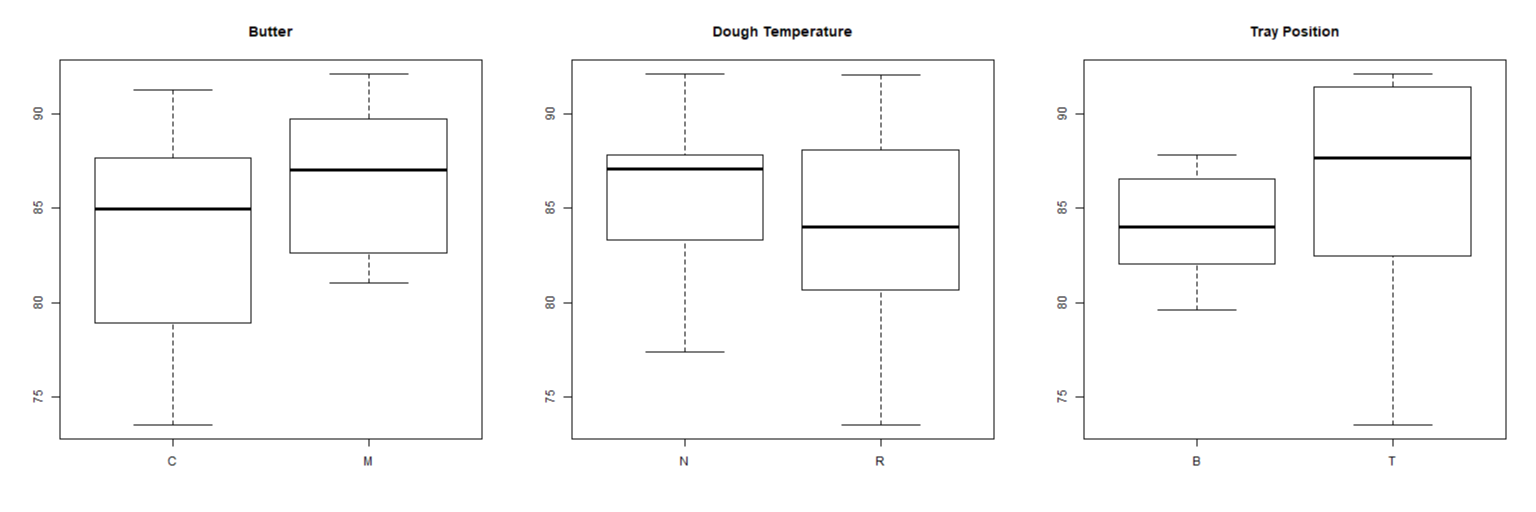
\includegraphics[width=.7\paperwidth]{boxplot-individuals}}
	\caption*{Figure 1: Individual Factor Effects on Cookie Size}
\end{figure}
\begin{figure}[H]
	\makebox[\textwidth][c]{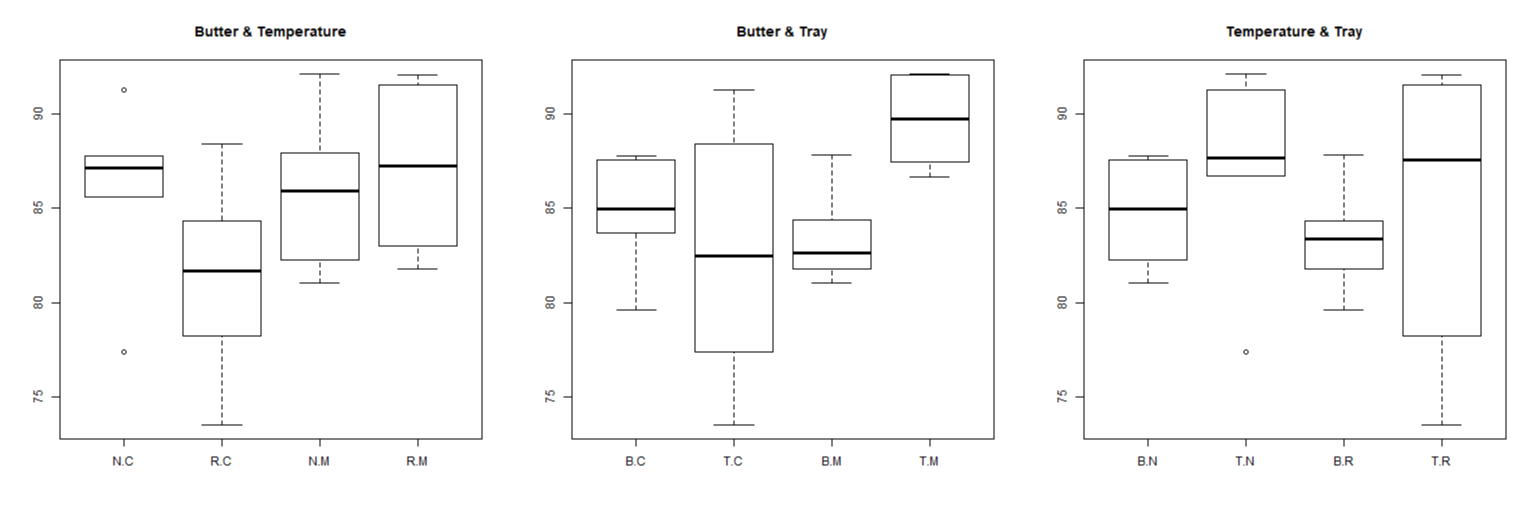
\includegraphics[width=.7\paperwidth]{boxplot-pairs}}
	\caption*{Figure 2: Pairwise Factor Effects on Cookie Size}
\end{figure}
\begin{figure}[H]
	\makebox[\textwidth][c]{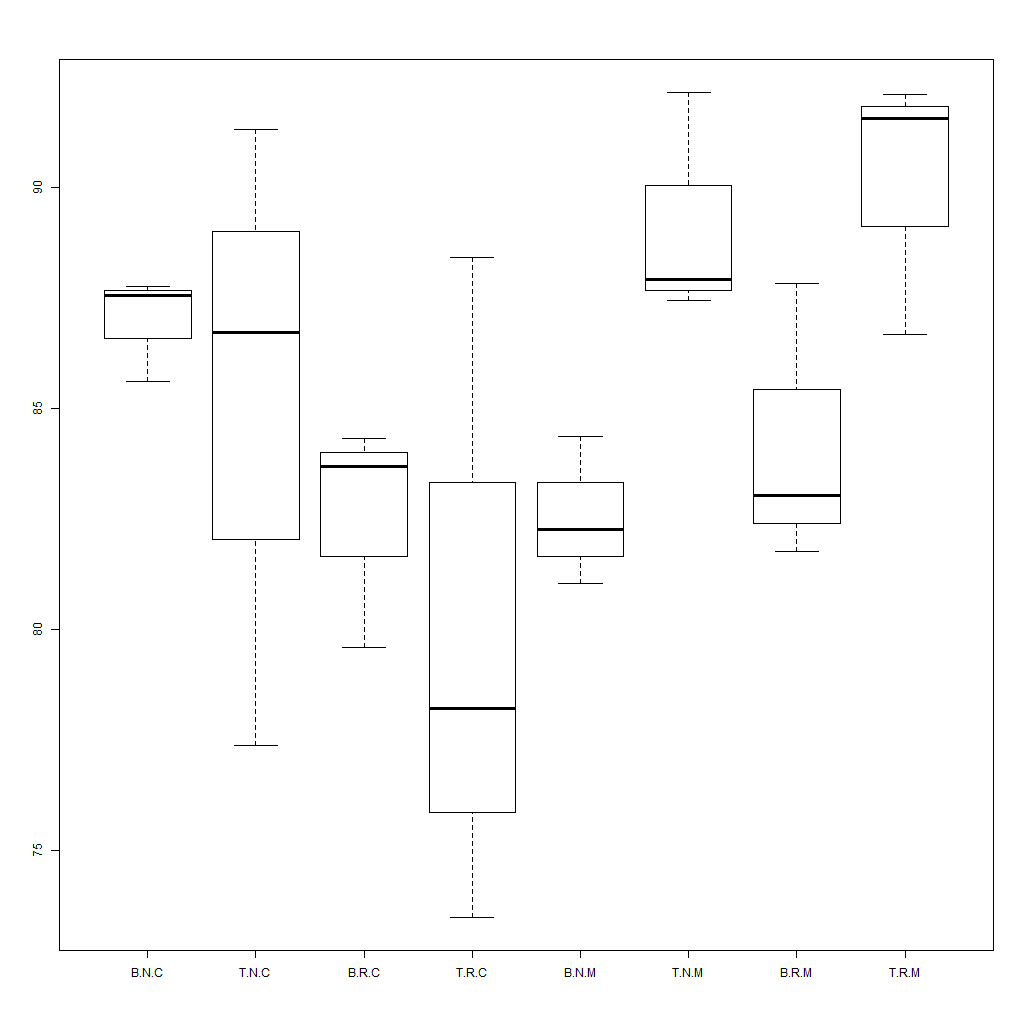
\includegraphics[width=.7\paperwidth]{boxplot-full}}
	\caption*{Figure 3: Full Factor Effects on Cookie Size}
\end{figure}

%----------------------------------------------------------------------------------------
%	Models
%----------------------------------------------------------------------------------------
\section*{\variableheghtrulefill[.25ex]\quad Model \quad\variableheghtrulefill[.25ex]}
Using the full model with all interactions, we can obtain the following model:
\begin{flalign*}
	Y_{b,d,t,c} & = \alpha_{b} + \beta_{d} + \gamma_{t} + \left(\alpha\beta\right)_{b,d} + \left(\alpha\gamma\right)_{b,t} + \left(\beta\gamma\right)_{dt} + \epsilon_{b,d,t,c}& \\
	\epsilon_{b,d,t,c} & \sim N(0, \sigma^2) &
\end{flalign*}

If one were to only examine the main effects, the ME model is as follows: 
\begin{flalign*}
	Y_{b,d,t,c} & = \alpha_{b} + \beta_{d} + \gamma_{t} + \epsilon_{b,d,t,c}& \\
	\epsilon_{b,d,t,c} & \sim N(0, \sigma^2) &
\end{flalign*}

%----------------------------------------------------------------------------------------
%	Analysis
%----------------------------------------------------------------------------------------
\section*{\variableheghtrulefill[.25ex]\quad R Analysis \quad\variableheghtrulefill[.25ex]}
Looking at the ANOVA table for the full model, we can see that the only truly significant factor is the interaction between the type of butter used and the tray position. The chilled dough and butter type interaction is significant if we relax our alpha value to 0.1.
\newpage
\lstinputlisting[language=, caption=Full Model ANOVA Table]{listings/project-FullAnova.txt}

For robustness, examining the full model yields the same result that the individual factors are not enough to result in a difference in the size of the cookies.

\lstinputlisting[language=, caption=Main Effects Model ANOVA Table]{listings/project-Main.txt}

Moving to check our normality assumptions, the below Q-Q and Residual vs Fitted Plots. The residual vs fitted plot shows relatively constant variance and there is nothing significantly out of place in the Q-Q plot to indicate that our normality assumptions are violated. The tails are both a bit skewed but the majority of the data is within a reasonable variance. Performing a log and square-root transformation on the data yielded minimal change in the normality plots, so the unaltered model was used.

\begin{figure}[H]
	\makebox[\textwidth][c]{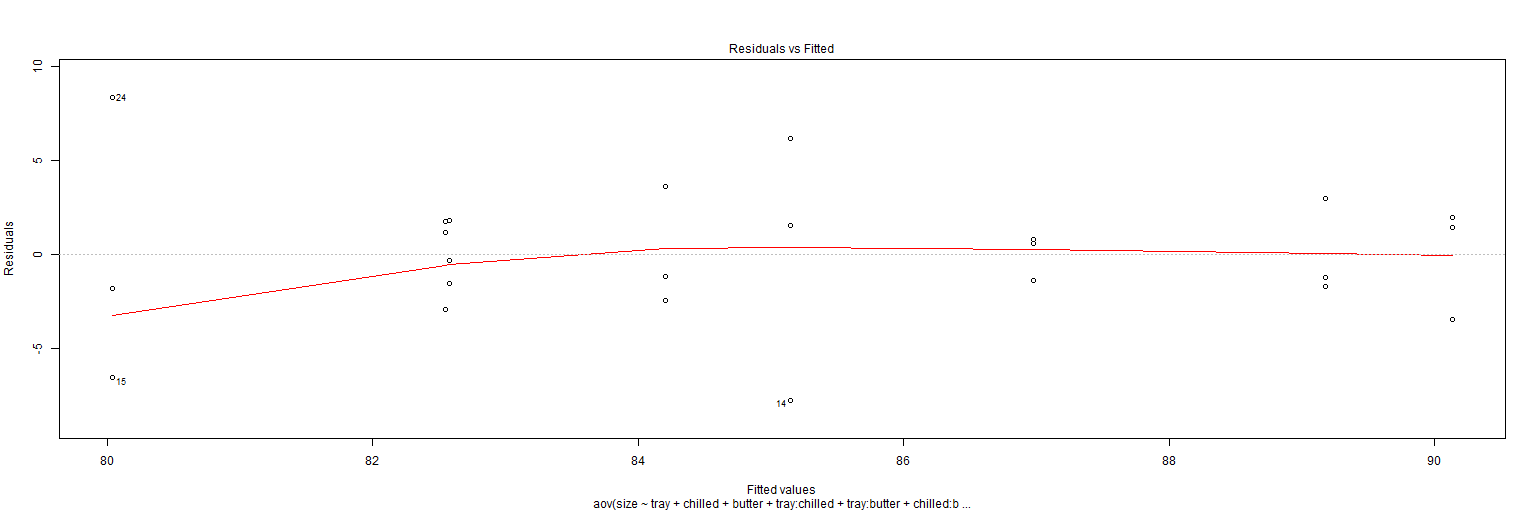
\includegraphics[width=.7\paperwidth]{normality-residuals}}
	\caption*{Figure 4: Residual vs Fitted Plot for Full Model}
\end{figure}
\begin{figure}[H]
	\makebox[\textwidth][c]{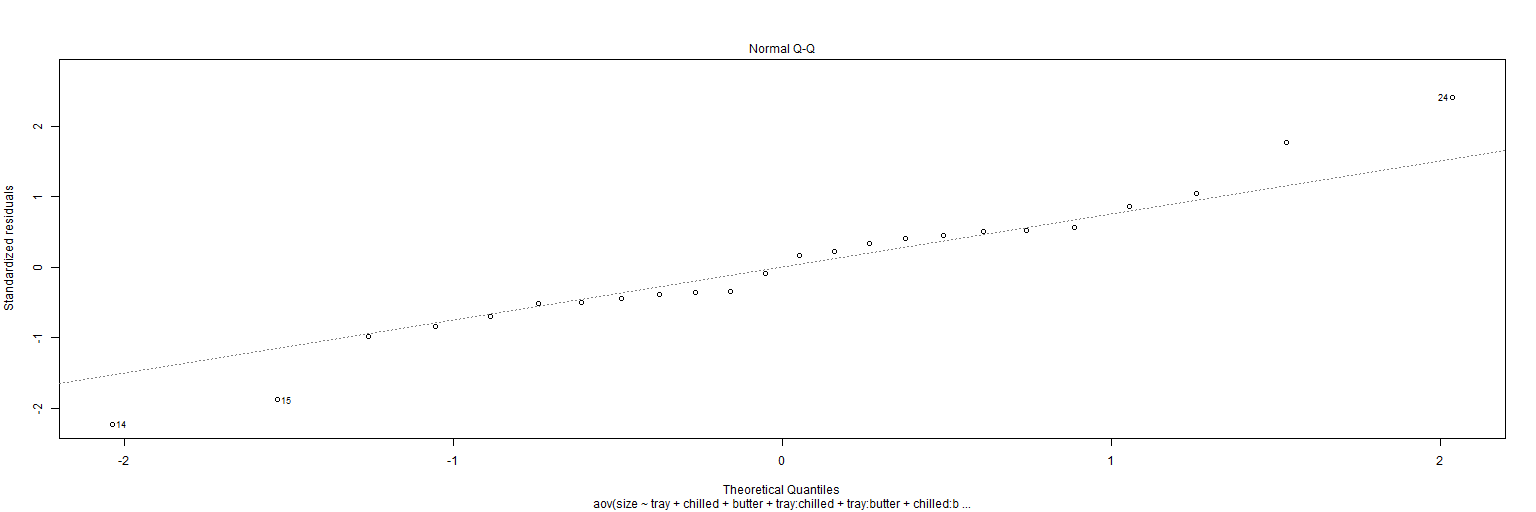
\includegraphics[width=.7\paperwidth]{normality-qq}}
	\caption*{Figure 5: Q-Q Plot for Full Model}
\end{figure}

Finally, because the only significant terms are interaction terms, an interaction plot was created for the two interaction pairs. These plots are below:

\begin{figure}[H]
	\makebox[\textwidth][c]{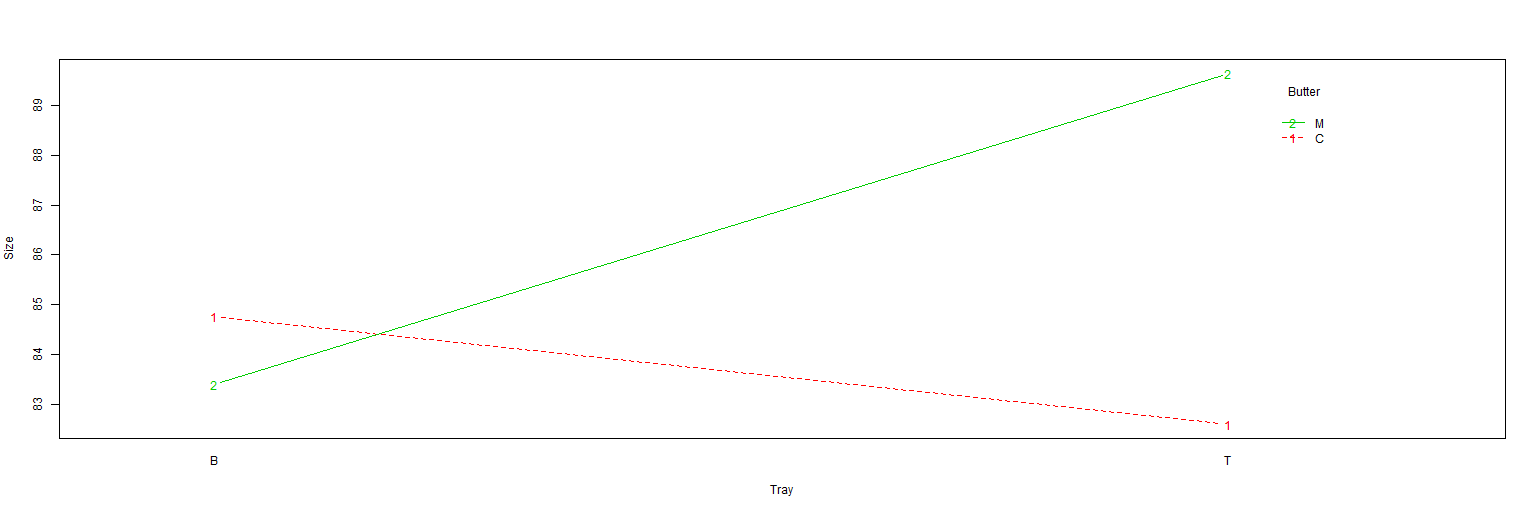
\includegraphics[width=.7\paperwidth]{interaction-tray-butter}}
	\caption*{Figure 6: (Tray Position:Butter Type) Interaction Plot}
\end{figure}
\begin{figure}[H]
	\makebox[\textwidth][c]{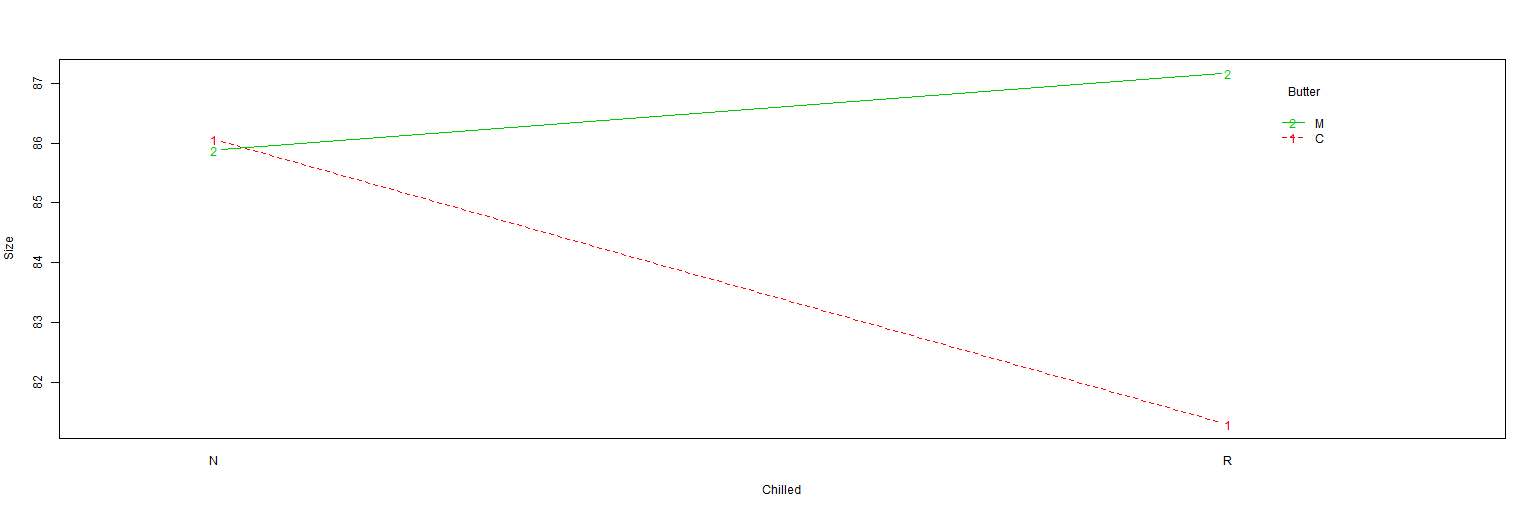
\includegraphics[width=.7\paperwidth]{interaction-chilled-butter}}
	\caption*{Figure 7: (Dough Temperature:Butter Type) Interaction Plot}
\end{figure}


\newpage
\section*{Data Appendix}
\begin{table}[H]
\centering
\begin{tabular}{|c|c|c|c|}
\hline
\textbf{Size (mm)} & \textbf{Butter} & \textbf{Dough Temperature} & \textbf{Tray Position} \\ \hline
85.61         & C               & N                & B             \\ \hline
87.56         & C               & N                & B             \\ \hline
83.03         & M               & R                & B             \\ \hline
87.78         & C               & N                & B             \\ \hline
81.78         & M               & R                & B             \\ \hline
83.70         & C               & R                & B             \\ \hline
84.32         & C               & R                & B             \\ \hline
87.83         & M               & R                & B             \\ \hline
82.28         & M               & N                & B             \\ \hline
81.06         & M               & N                & B             \\ \hline
79.60         & C               & R                & B             \\ \hline
84.38         & M               & N                & B             \\ \hline
91.32         & C               & N                & T             \\ \hline
77.38         & C               & N                & T             \\ \hline
73.49         & C               & R                & T             \\ \hline
78.23         & C               & R                & T             \\ \hline
86.69         & M               & R                & T             \\ \hline
87.93         & M               & N                & T             \\ \hline
86.72         & C               & N                & T             \\ \hline
87.45         & M               & N                & T             \\ \hline
91.57         & M               & R                & T             \\ \hline
92.12         & M               & R                & T             \\ \hline
92.17         & M               & N                & T             \\ \hline
88.42         & C               & R                & T             \\ \hline
\end{tabular}
\caption*{Table of Collected Data}
\end{table}

\newpage
\section*{Code Appendix}
\lstinputlisting[language=R]{project.R}

\end{document}